\documentclass[12pt]{kiarticle} % You can learn about my document class "kiarticle" and install it to your device by following the link: https://github.com/Kiarendil/toolkitex
\graphicspath{{pictures/}}
\DeclareGraphicsExtensions{.pdf,.png,.jpg,.eps}
%%%
\pagestyle{fancy}
\fancyhf{}
%\renewcommand{\headrulewidth}{ 0.1mm }
\renewcommand{\footrulewidth}{ .0em }
\fancyfoot[C]{\texttt{\textemdash~\thepage~\textemdash}}
\fancyhead[L]{Лабораторная работа № 4.3.2 \hfil}
\fancyhead[R]{\hfil Иванов Кирилл, 625 группа }
\usepackage{multirow} % Слияние строк в таблице
\newcommand
{\un}[1]
{\ensuremath{\text{#1}}}
\newcommand{\eds}{\ensuremath{ \mathscr{E}}}
\usepackage{tikz}
%%% Работа с таблицами
\usepackage{array,tabularx,tabulary,booktabs} % Дополнительная работа с таблицами
\usepackage{longtable}  % Длинные таблицы
\usepackage{multirow} % Слияние строк в таблице
\newcommand{\specialcell}[2][c]{%
	\begin{tabular}[#1]{@{}c@{}}#2\end{tabular}}

\begin{document}
	
	\begin{titlepage}
	\begin{center}
		\large 	Московский физико-технический институт \\
		(государственный университет) \\
		Факультет общей и прикладной физики \\
		\vspace{0.2cm}
		
		\vspace{4.5cm}
		Лабораторная работа № 4.3.2 \\ \vspace{0.2cm}
		\large (Общая физика: оптика) \\ \vspace{0.2cm}
		\LARGE \textbf{Дифракция света на ультразвуковой волне в жидкости}
	\end{center}
	\vspace{2.3cm} \large
	
	\begin{center}
		Работу выполнил: \\
		Иванов Кирилл,
		625 группа
		\vspace{10mm}		
		
	\end{center}
	
	\begin{center} \vspace{60mm}
		г. Долгопрудный \\
		2018 год
	\end{center}
\end{titlepage}
	
	\paragraph*{Цель работы:} изучение дифракции света на синусоидальной акустической решетке и
	наблюдение фазовой решетки методом темного поля.
	
	\paragraph*{Оборудование:} оптическая скамья, осветитель, два длиннофокусных объектива, кювета с жидкостью, кварцевый излучатель с микрометрическим винтом, генератор звуковой частоты, линза, вертикальная нить на рейтере, микроскоп.
	
	\section{Теоретическое введение}
	
	В работе используются оптическая скамья, осветитель, два длиннофокусных объектива, кювета с жидкостью, кварцевый излучатель с микрометрическим винтом, генератор звуковой частоты, линза, горизонтальная нить на рейтере, микроскоп. 
	
	При прохождении ультразвуковой волны через жидкость в ней возникают периодические неоднородности коэффициента преломления, создается фазовая решетка, которую мы считаем неподвижной ввиду малости скорости звука относительно скорости света. Показатель
	преломления n изменяется по закону:
	
	\begin{equation}\label{}
	n = n_0 (1 + m \cos \Omega x)
	\end{equation}
	
	Здесь $ \Omega = 2 \pi / \Lambda $ --- волновое число для ультразвуковой волны, $ m $ --- глубина модуляции $ n $ $ (m \ll 1 $).
	
	Положим фазу $ \phi $ колебаний световой волны на передней стенке кюветы равной нулю, тогда на задней поверхности она равна:
	
	\begin{equation}\label{}
	\phi  = k n L = \phi_0 (1 + m \cos \Omega x)
	\end{equation}
	
	Здесь $ L $ --- толщина жидкости в кювете, $ k = 2 \pi / \lambda $ --- волновое число для света.
	
	После прохождения через кювету световое поле есть совокупность плоских волн, распространяющихся под углами $ \theta $, соответствующими максимумам в дифракции Фраунгофера:
	
\begin{equation}\label{}	
	\Lambda \sin \theta_m = m \lambda
\end{equation}

	Этот эффект проиллюстрирован на рисунке 1.
	\begin{figure}[h!]
		\centering	
		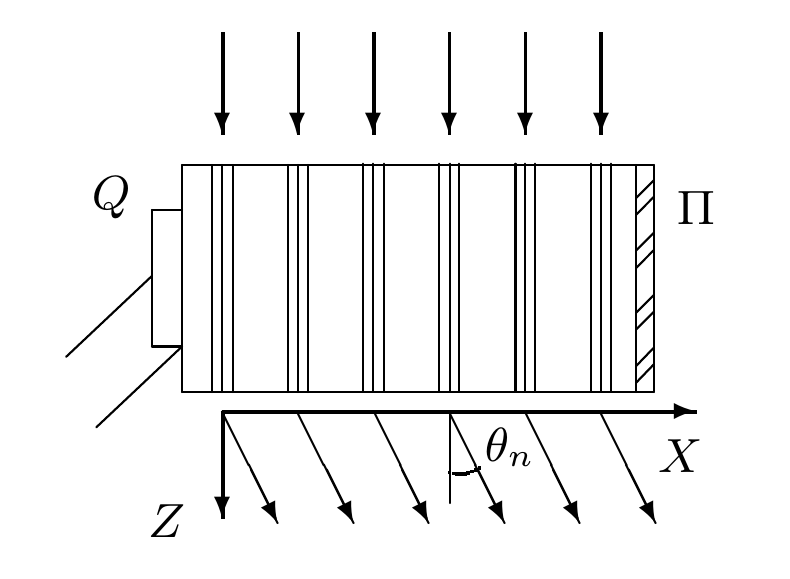
\includegraphics[width=0.3\textwidth]{difraction.png}
		\caption{Дифракция световых волн на акустической решетке}
		\label{diff}
	\end{figure}

	Зная положение дифракционных максимумов, по формуле (1) легко определить длину ультразвуковой волны, учитывая малость $ \theta $: $ \sin \theta \approx \theta \approx l_m /F  $, где $ l_m $ --- расстояние от нулевого до последнего видимого максимума, $ F $ --- фокусное расстояние линзы. Тогда получим:
	
	\begin{equation}\label{}
	 \Lambda = m \lambda F/ l_m 
	\end{equation}
	Скорость ультразвуковых волн в жидкости, где $ \nu $ --- частота колебаний излучателя:
	
\begin{equation}\label{}
	v = \Lambda \nu 
\end{equation}

\section{Определение скорости ультразвука по дифракционной картине}

Схема установки приведена на рисунке 2. Источник света Л через светофильтр Ф и конденсор К освещает вертикальную щель $ S $, находящуюся в фокусе объектива $ O_1 $. После объектива параллельный световой пучок проходит через кювету С перпендикулярно акустической решетке, и дифракционная картина собирается в фокальной плоскости объектива $ O_2 $ , наблюдается при помощи микроскопа М.

Предварительную настройку установки произведем в соответствии с инструкцией с зеленым фильтром, далее в работе используется красный.

	\begin{figure}[h!]
	\centering	
	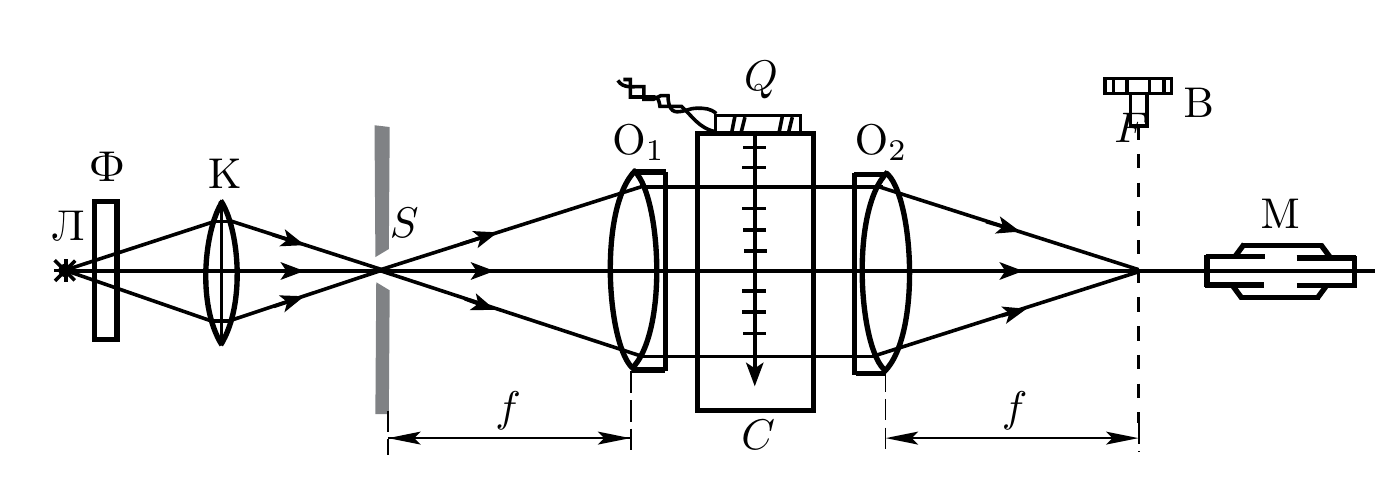
\includegraphics[width=0.7\textwidth]{shema1.png}
	\caption{Схема для наблюдения дифракции на акустической решетке}
	\label{shema1}
\end{figure}

Параметры установки: фокусное расстояние объектива $  O_2  $ $ F = 30 $ см, одно деление винта микроскопа составляет 4 мкм, погрешность измерений примем равной  $ \sigma = $ 2 деления, или 8 мкм.

Исследуем изменения дифракционной картины на зеленом свете. При увеличении частоты УЗ-генератора и приближении к 1,1 МГц проявляется дифракционная решетка: расстояние между максимумами растет.

Измерим положения $ x_m $ дифракционных максимумов с помощью микроскопического винта для четырех частот. Результаты измерений занесены в таблицы 1-4 ниже. На основе каждой таблицы построены графики зависимости $ x_m (m) $, они изображены на рисунках 3-6. Коэффициенты углов наклонов прямых для всех зависимостей сведены в таблицу 5. 

	\begin{table}[h!]
	\centering
	\begin{tabular}{|c|c|c|c|c|c|c|c|}
\hline
$m$&-3&-2&-1&0&1&2&3\\
\hline
$x_m$, дел&-115&-78&-37&0&38&74&106\\
\hline
$x_m$, мкм&-460&-312&-148&0&152&296&424\\
\hline
\end{tabular}

	\caption{Измерение координаты $ m $-ого максимума $ x_m $ дифракционной картины при частоте генератора $ \nu = $ 1,168 МГц}
	\label{nu1}
\end{table}	

	\begin{figure}[h!]
	\centering
	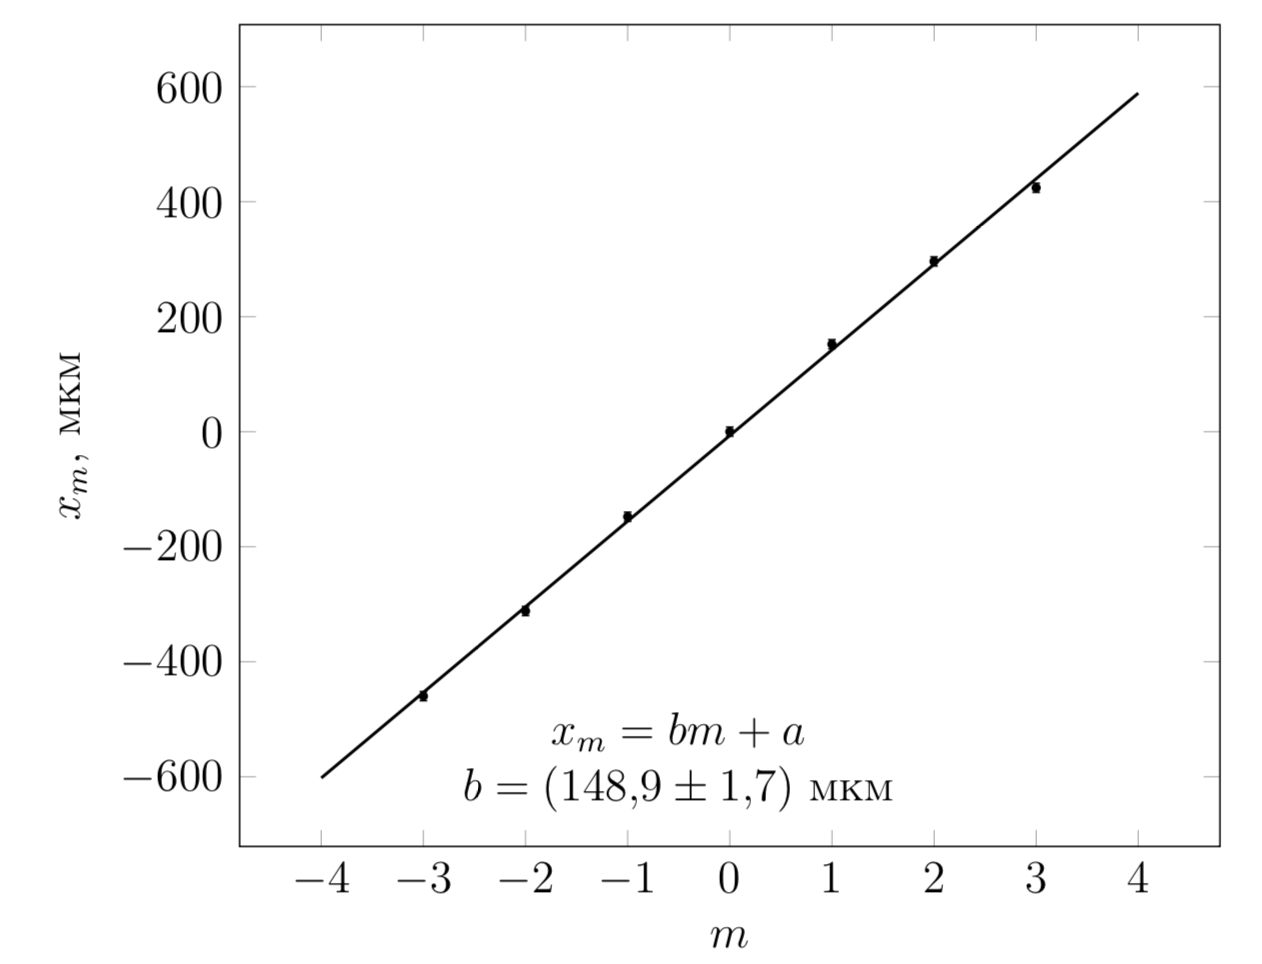
\includegraphics[width=0.7\linewidth]{1.png}
	\caption{График зависимость$  x_m(m) $ при частоте генератора $ \nu = $ 1,168 МГц}
	\label{nu1_graf}
\end{figure}
	
		\begin{table}[h!]
		\centering
		\begin{tabular}{|c|c|c|c|c|c|c|c|c|c|}
\hline
$m$&-4&-3&-2&-1&0&1&2&3&4\\
\hline
$x_m$, дел&-150&-116&-81&-38&0&38&80&120&154\\
\hline
$x_m$, мкм&-600&-464&-324&-152&0&152&320&480&616\\
\hline
\end{tabular}

		\caption{Измерение координаты $ m $-ого максимума $ x_m $ дифракционной картины при частоте генератора $ \nu = $ 1,219 МГц}
		\label{nu2}
	\end{table}	

\begin{figure}[h!]
	\centering
	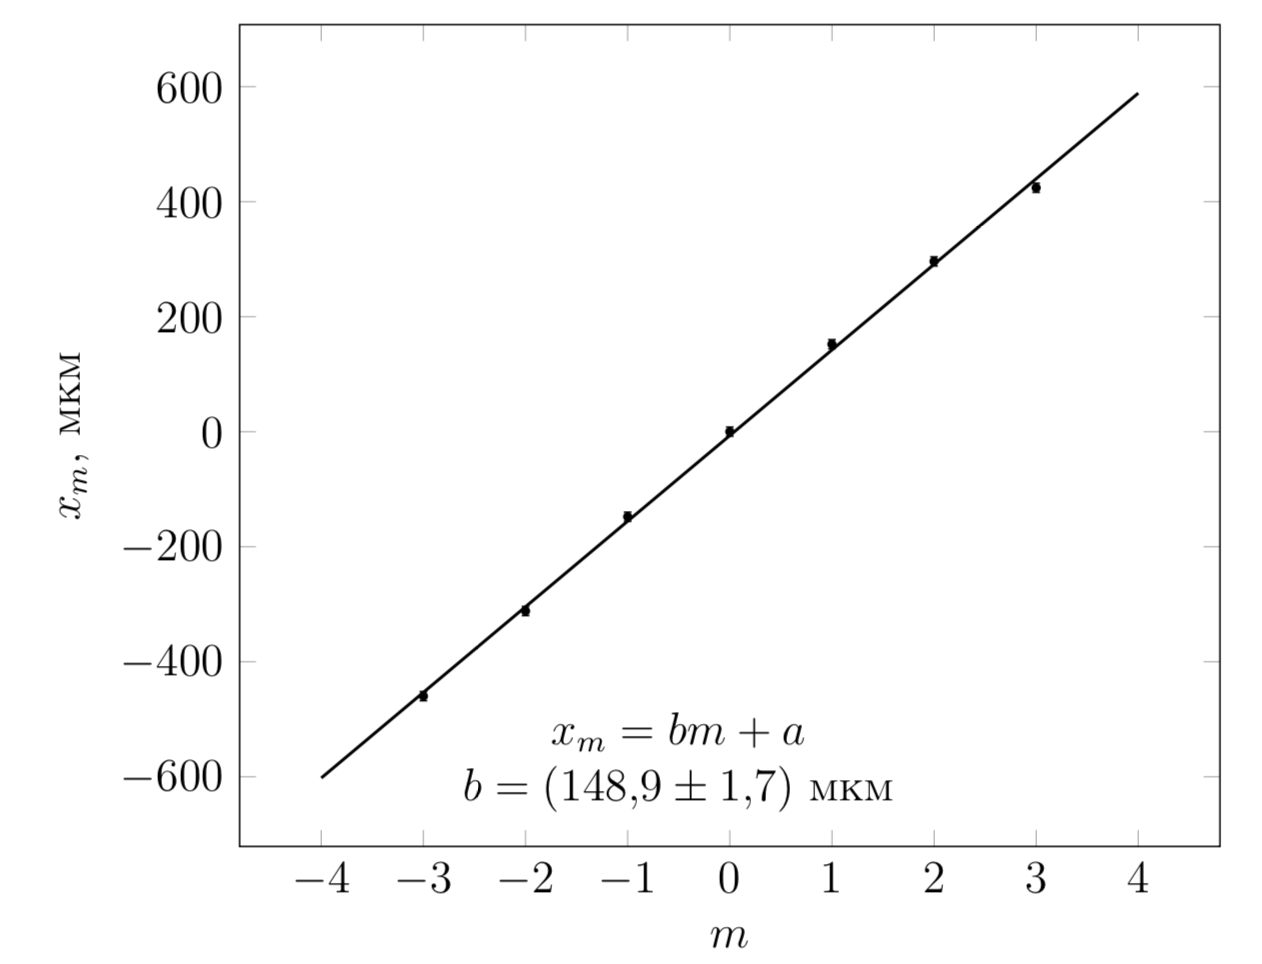
\includegraphics[width=0.7\linewidth]{1.png}
	\caption{График зависимость$  x_m(m) $ при частоте генератора $ \nu = $ 1,219 МГц}
	\label{nu2_graf}
\end{figure}

		\begin{table}[h!]
		\centering
		\begin{tabular}{|c|c|c|c|c|c|c|c|}
\hline
$m$&-3&-2&-1&0&1&2&3\\
\hline
$x_m$, дел&-116&-80&-38&0&45&86&126\\
\hline
$x_m$, мкм&-464&-320&-152&0&180&344&504\\
\hline
\end{tabular}
		\caption{Измерение координаты $ m $-ого максимума $ x_m $ дифракционной картины при частоте генератора $ \nu = $ 1,248 МГц}
		\label{nu3}
	\end{table}	

\begin{figure}[h!]
	\centering
	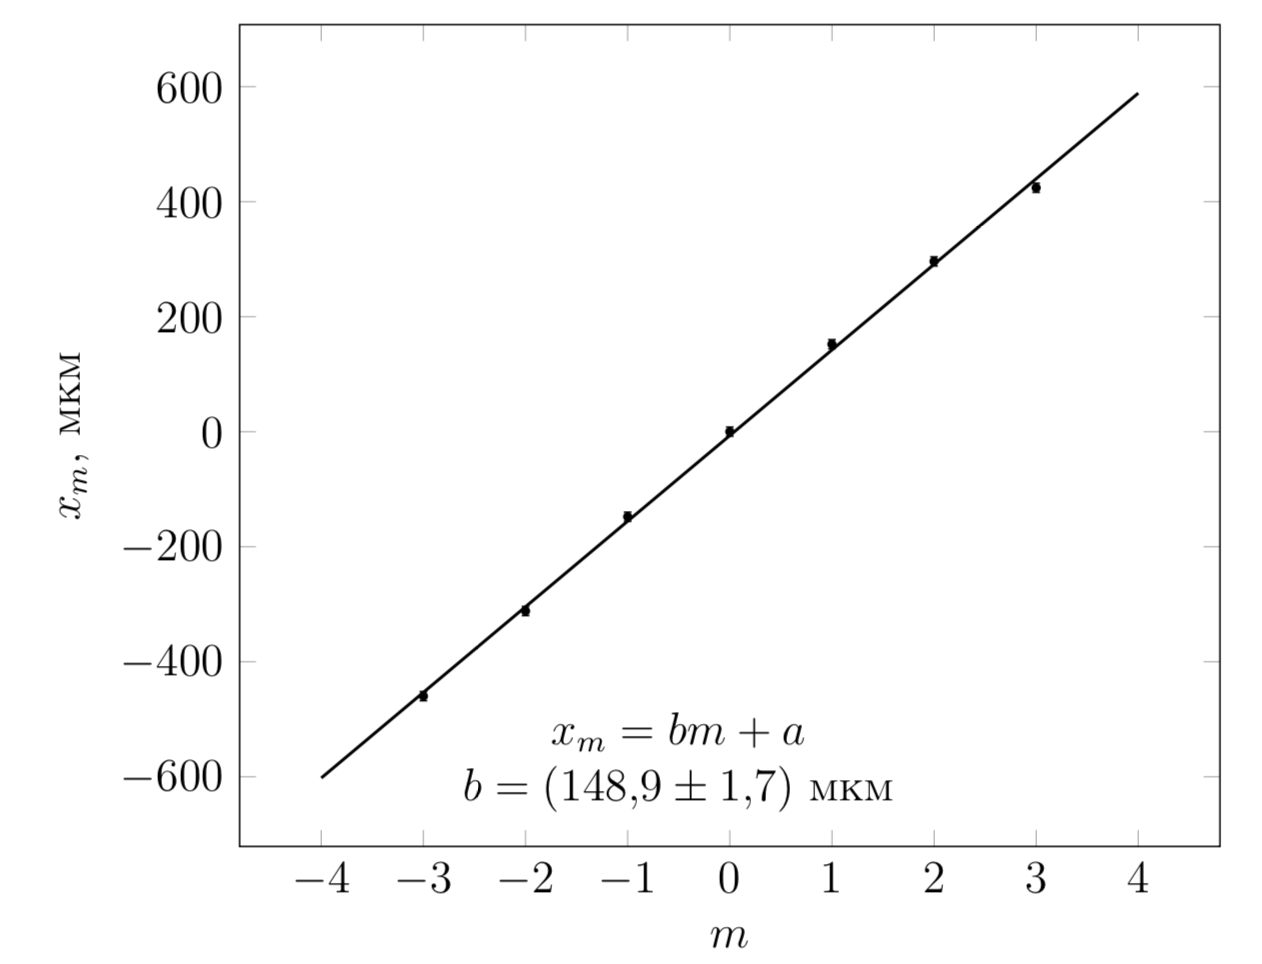
\includegraphics[width=0.7\linewidth]{1.png}
	\caption{График зависимость$  x_m(m) $ при частоте генератора $ \nu = $ 1,248 МГц}
	\label{nu3_graf}
\end{figure}

	\begin{table}[h!]
	\centering
	\begin{tabular}{|c|c|c|c|c|c|}
\hline
$m$&-2&-1&0&1&2\\
\hline
$x_m$, дел&-94&-43&0&45&85\\
\hline
$x_m$, мкм&-376&-172&0&180&340\\
\hline
\end{tabular}
	\caption{Измерение координаты $ m $-ого максимума $ x_m $ дифракционной картины при частоте генератора $ \nu = $ 1,331 МГц}
	\label{nu4}
\end{table}	

\begin{figure}[h!]
	\centering
	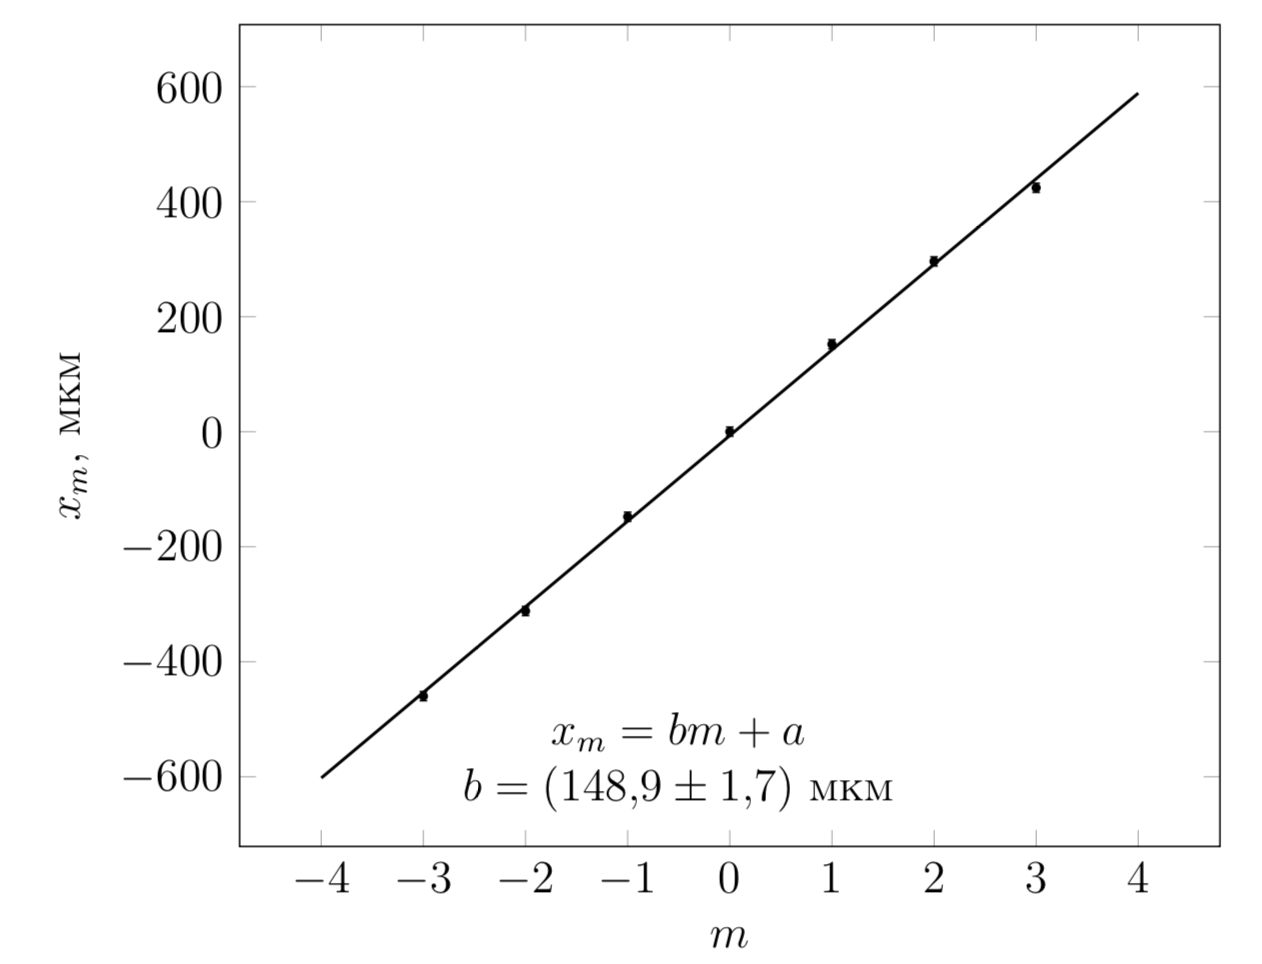
\includegraphics[width=0.7\linewidth]{1.png}
	\caption{График зависимость$  x_m(m) $ при частоте генератора $ \nu = $ 1,331 МГц}
	\label{nu4_graf}
\end{figure}

	\begin{table}[h!]
	\centering
	\begin{tabular}{|c|c|c|c|c|c|c|c|c|c|c|}
\hline
$\nu$, МГц&$b$, мкм&$\sigma_b$, мкм&$\Lambda$, мкм&$\Delta \Lambda$, мкм&$v$, м/с&$\Delta v$, м/с\\
\hline
1,168&148,9&1,7&1289&15&1507&17\\
\hline
1,219&154,8&1,3&1240&10&1512&12\\
\hline
1,258&163,0&1,4&1178&10&1482&13\\
\hline
1,331&178&3&1076&19&1432&26\\
\hline
\end{tabular}
	\caption{Вычисление длины ультразвуковой волны $ \Lambda $ и скорости распространения ее в воде $ v $}
	\label{speed}
\end{table}	

\newpage

Ошибка при определении $ \Lambda $ и $ v $ не превышает 2\%. Согласно справочным данным, при комнатной температуре скорость ультразвуковой волны в воде составляет примерно 1490 м/с. Значения, полученные экспериментально, с достаточной точностью соотносятся с ними.

\newpage

\section{Определение скорости ультразвука методом темного поля}

Для наблюдения акустической решетки используется метод темного поля, который заключается в устранении центрального дифракционного максимума с помощью непрозрачного экрана. Схема установки показана на рисунке 7.

	\begin{figure}[h!]
	\centering	
	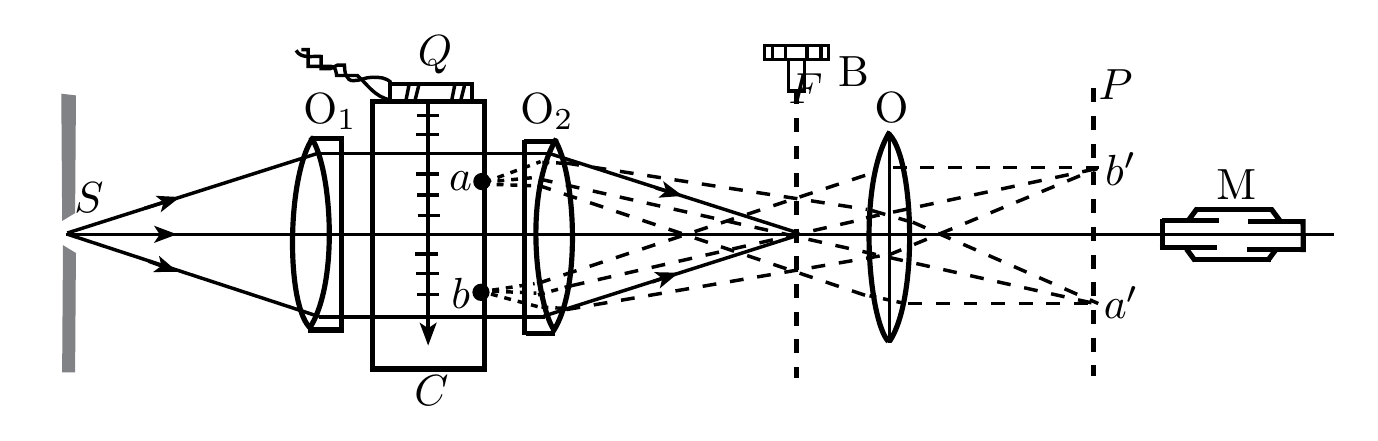
\includegraphics[width=0.7\textwidth]{shema2.png}
	\caption{Схема для наблюдения дифракции методом темного поля}
	\label{shema2}
\end{figure}

Приставим к задней стенке (для светового луча) кюветы стеклянную пластинку с миллиметровыми делениями; сфокусируем микроскоп на изображение пластинки. Определим цену деления окулярной шкалы микроскопа, совместив ее с миллиметровыми делениями: в 6 делениях миллиметровой шкалы убирается 100 маленьких делений окулярной. Значит, цена деления окулярной шкалы: $ C = $ 0,06 мм.

Без применения метода темного поля звуковая решетка не наблюдается. Закроем нулевой максимум горизонтальной нитью. Таким образом, осевая составляющая фазово-модулированной волны поглощается, а боковые остаются без изменения. Получившееся поле: 

\begin{equation}\label{}
f(x) = \dfrac{im}{2} e^{i\Omega x} +  \dfrac{im}{2} e^{-i\Omega x} = im \cos \Omega x \te I(x) = m^2 \cos ^2 \Omega x = m^2 \dfrac{1 + \cos ^2 2 \Omega x}{2}
\end{equation}

Отсюда получаем, что расстояние между темными полосами есть $ \Lambda/2 $.

Проведем измерение длины ультразвуковой волны, приняв ошибку равной цене деления окулярной шкалы. В таблице 6 содержатся количество маленьких делений окулярной шкалы N (цена деления $ C = 0,06 $), соответствующее $ n $ темным полосам акустической решетки.
Формулы для расчета длины волны ультразвука $ \Lambda $ и скорости распространения $ v $ в воде:
\begin{equation}\label{}
\Lambda/2  = NC/(n - 1),  \qquad v = \nu\Lambda
\end{equation}

Расчеты также приведены в таблице 6. Ошибка при таком определении скорости звука больше, чем в первой части работы, и
составляет около 5\%. Сами значения тоже получились больше.


\begin{table}[h!]
	\centering
	\begin{tabular}{|c|c|c|c|c|c|c|c|c|c|}
\hline
$\nu$, Мгц& \specialcell{Количество делений \\ шкалы окуляра $N$}&\specialcell{Количество темных полос \\ акустической решетки $n$}&$\Lambda$, мм&$v$, $10$ м/с&$\Delta v$, $10$ м/с\\
\hline
1,220&150&15&1,29&157&7\\
\hline
1,259&150&16&1,20&151&8\\
\hline
1,271&175&18&1,24&157&8\\
\hline
\end{tabular}

	\caption{Вычисление длины ультразвуковой волны $ \Lambda $ и скорости распространения ее в воде $ v $ методом темного поля}
	\label{dark}
\end{table}	

\section{Вывод}

В работе изучена дифракция света на акустической решетки, рассчитаны длина волны ультразвука и скорость его распространения в воде. Решетка наблюдалась методом
темного поля.

	
\end{document}